% Options for packages loaded elsewhere
\PassOptionsToPackage{unicode}{hyperref}
\PassOptionsToPackage{hyphens}{url}
\PassOptionsToPackage{dvipsnames,svgnames,x11names}{xcolor}
%
\documentclass[
  12pt,
]{article}
\title{~\Large Eras in baseball: Change point analysis fun title.}
\author{\large Mena Whalen \vspace{-1.1mm}\\
\normalsize Department of Mathematics and Statistics \vspace{-1mm}\\
\normalsize Loyola University Chicago \vspace{-1mm}\\
\normalsize Chicago, IL 60660 \vspace{-1mm}\\
\normalsize \href{mailto:mwhalen3@luc.edu}{\texttt{mwhalen3@luc.edu}}
\vspace{-1mm}\\
\strut \\
\large Gregory J. Matthews \vspace{-1.1mm}\\
\normalsize Department of Mathematics and Statistics \vspace{-1mm}\\
\normalsize Loyola University Chicago \vspace{-1mm}\\
\normalsize Chicago, IL 60660 \vspace{-1mm}\\
\normalsize \href{mailto:gmatthews1@luc.edu}{\texttt{gmatthews1@luc.edu}}
\vspace{-1mm}}
\date{}

\usepackage{amsmath,amssymb}
\usepackage{lmodern}
\usepackage{iftex}
\ifPDFTeX
  \usepackage[T1]{fontenc}
  \usepackage[utf8]{inputenc}
  \usepackage{textcomp} % provide euro and other symbols
\else % if luatex or xetex
  \usepackage{unicode-math}
  \defaultfontfeatures{Scale=MatchLowercase}
  \defaultfontfeatures[\rmfamily]{Ligatures=TeX,Scale=1}
\fi
% Use upquote if available, for straight quotes in verbatim environments
\IfFileExists{upquote.sty}{\usepackage{upquote}}{}
\IfFileExists{microtype.sty}{% use microtype if available
  \usepackage[]{microtype}
  \UseMicrotypeSet[protrusion]{basicmath} % disable protrusion for tt fonts
}{}
\makeatletter
\@ifundefined{KOMAClassName}{% if non-KOMA class
  \IfFileExists{parskip.sty}{%
    \usepackage{parskip}
  }{% else
    \setlength{\parindent}{0pt}
    \setlength{\parskip}{6pt plus 2pt minus 1pt}}
}{% if KOMA class
  \KOMAoptions{parskip=half}}
\makeatother
\usepackage{xcolor}
\IfFileExists{xurl.sty}{\usepackage{xurl}}{} % add URL line breaks if available
\IfFileExists{bookmark.sty}{\usepackage{bookmark}}{\usepackage{hyperref}}
\hypersetup{
  colorlinks=true,
  linkcolor={cyan},
  filecolor={Maroon},
  citecolor={Blue},
  urlcolor={cyan},
  pdfcreator={LaTeX via pandoc}}
\urlstyle{same} % disable monospaced font for URLs
\usepackage[margin=1in]{geometry}
\usepackage{graphicx}
\makeatletter
\def\maxwidth{\ifdim\Gin@nat@width>\linewidth\linewidth\else\Gin@nat@width\fi}
\def\maxheight{\ifdim\Gin@nat@height>\textheight\textheight\else\Gin@nat@height\fi}
\makeatother
% Scale images if necessary, so that they will not overflow the page
% margins by default, and it is still possible to overwrite the defaults
% using explicit options in \includegraphics[width, height, ...]{}
\setkeys{Gin}{width=\maxwidth,height=\maxheight,keepaspectratio}
% Set default figure placement to htbp
\makeatletter
\def\fps@figure{htbp}
\makeatother
\setlength{\emergencystretch}{3em} % prevent overfull lines
\providecommand{\tightlist}{%
  \setlength{\itemsep}{0pt}\setlength{\parskip}{0pt}}
\setcounter{secnumdepth}{5}
\newlength{\cslhangindent}
\setlength{\cslhangindent}{1.5em}
\newlength{\csllabelwidth}
\setlength{\csllabelwidth}{3em}
\newlength{\cslentryspacingunit} % times entry-spacing
\setlength{\cslentryspacingunit}{\parskip}
\newenvironment{CSLReferences}[2] % #1 hanging-ident, #2 entry spacing
 {% don't indent paragraphs
  \setlength{\parindent}{0pt}
  % turn on hanging indent if param 1 is 1
  \ifodd #1
  \let\oldpar\par
  \def\par{\hangindent=\cslhangindent\oldpar}
  \fi
  % set entry spacing
  \setlength{\parskip}{#2\cslentryspacingunit}
 }%
 {}
\usepackage{calc}
\newcommand{\CSLBlock}[1]{#1\hfill\break}
\newcommand{\CSLLeftMargin}[1]{\parbox[t]{\csllabelwidth}{#1}}
\newcommand{\CSLRightInline}[1]{\parbox[t]{\linewidth - \csllabelwidth}{#1}\break}
\newcommand{\CSLIndent}[1]{\hspace{\cslhangindent}#1}
\usepackage{setspace} \setstretch{1.15} \usepackage{float} \floatplacement{figure}{t}
\ifLuaTeX
  \usepackage{selnolig}  % disable illegal ligatures
\fi

\begin{document}
\maketitle
\begin{abstract}
Baseball is some weird and wild shit. \vspace{2mm}\\
\emph{Keywords}: change point analysis, baseball,
\end{abstract}

\newpage

\hypertarget{sec:intro}{%
\section{Introduction}\label{sec:intro}}

\protect\hyperlink{ref-Berry1999bridging}{Berry, Reese, and Larkey}
(\protect\hyperlink{ref-Berry1999bridging}{1999}) they talk about
bridging eras.

When did the steroids era start:
\url{https://www.espn.com/mlb/topics/_/page/the-steroids-era\#}:\textasciitilde:text=Unlike\%20other\%20MLB\%20\%22eras\%2C\%22,leaguewide\%20PED\%20testing\%20until\%202003.

Traditional wisdom: 1900-1919 dead ball era

From Woltring: ``Baseball has endured much change over the course of its
history, and because of constant change, the modern era of baseball has
been segmented into six distinct sub-eras. A common list presented at
Baseball-Reference described the eras as the Dead Ball Era (1901-1919),
the Live Ball Era (1920-1941), the Integration Era (1942-1960), the
Expansion Era (1961-1976), the Free Agency Era (1977-1993) and the Long
Ball/Steroid Era (1994-2005) (17). This study runs through the 2011
season and a seventh era will be added and labeled the Post Steroid Era
(2006-2011)''

\url{https://www.baseball-reference.com/bullpen/Deadball_Era} 1901-1920

Mound was lowered in december 1968.\\
\url{https://www.baseball-reference.com/bullpen/Pitcher\%27s_mound}

\url{https://www.espn.com/mlb/story/_/id/33238595/major-league-baseball-stops-testing-players-steroids-nearly-20-years-report-says}

\hypertarget{methods}{%
\section{Methods}\label{methods}}

\protect\hyperlink{ref-ChoFryzlewwicz2014}{H. Cho and Fryzlewicz}
(\protect\hyperlink{ref-ChoFryzlewwicz2014}{2014}) and
\protect\hyperlink{ref-Cho2016}{H. Cho}
(\protect\hyperlink{ref-Cho2016}{2016})

R Pacakge: \protect\hyperlink{ref-hdbinseg}{Haeran Cho and Fryzlewicz}
(\protect\hyperlink{ref-hdbinseg}{2018})

\hypertarget{results}{%
\section{Results}\label{results}}

\begin{verbatim}
## [1] 20 46 67 94
\end{verbatim}

\begin{verbatim}
##  b 
## 48
\end{verbatim}

\begin{center}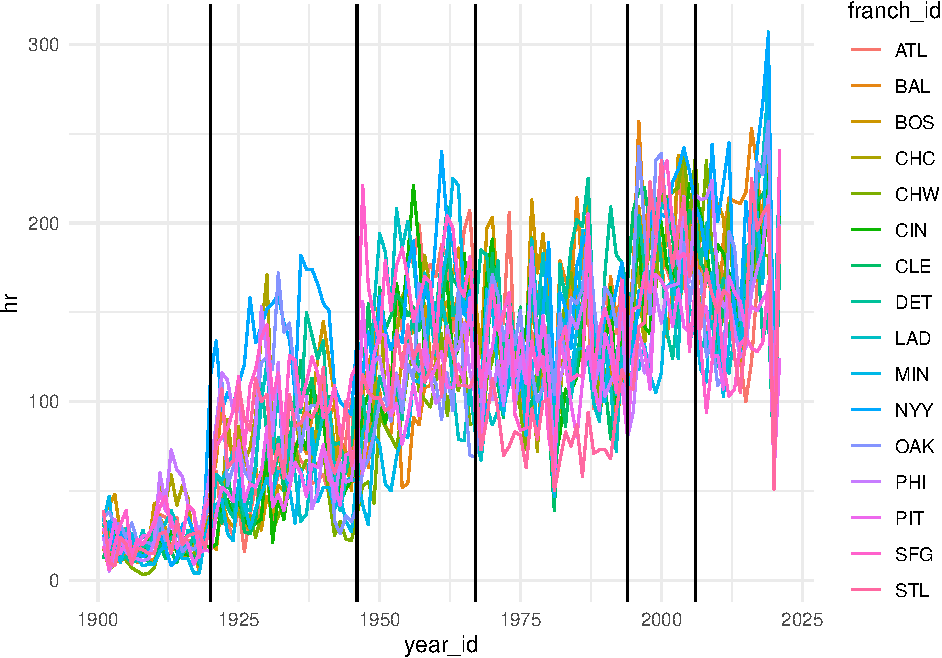
\includegraphics{paper_files/figure-latex/unnamed-chunk-1-1} \end{center}

\hypertarget{acknowledgements}{%
\section*{Acknowledgements}\label{acknowledgements}}
\addcontentsline{toc}{section}{Acknowledgements}

We thank Michael Lopez for suggesting we do ``something with change
point analysis.''

\hypertarget{supplementary-material}{%
\section*{Supplementary Material}\label{supplementary-material}}
\addcontentsline{toc}{section}{Supplementary Material}

All code for reproducing the analyses in this paper is publicly
available at \url{https://github.com/menawhalen/baseball_cpt}

\hypertarget{references}{%
\section*{References}\label{references}}
\addcontentsline{toc}{section}{References}

\hypertarget{refs}{}
\begin{CSLReferences}{1}{0}
\leavevmode\vadjust pre{\hypertarget{ref-Berry1999bridging}{}}%
Berry, Scott M., C. Shane Reese, and Patrick D. Larkey. 1999.
{``Bridging Different Eras in Sports.''} \emph{Journal of the American
Statistical Association} 94 (447): 661--76.
\url{https://doi.org/10.1080/01621459.1999.10474163}.

\leavevmode\vadjust pre{\hypertarget{ref-Cho2016}{}}%
Cho, H. 2016. {``Change-Point Detection in Panel Data via Double CUSUM
Statistic.''} \emph{Electronic Journal of Statistics} 10: 2000--2038.

\leavevmode\vadjust pre{\hypertarget{ref-hdbinseg}{}}%
Cho, Haeran, and Piotr Fryzlewicz. 2018. \emph{Hdbinseg: Change-Point
Analysis of High-Dimensional Time Series via Binary Segmentation}.
\url{https://CRAN.R-project.org/package=hdbinseg}.

\leavevmode\vadjust pre{\hypertarget{ref-ChoFryzlewwicz2014}{}}%
Cho, H., and P. Fryzlewicz. 2014. {``Multiple-Change-Point Detection for
High Dimensional Time Series via Sparsified Binary Segmentation.''}
\emph{JRSSB} 77: 475--507.

\end{CSLReferences}

\end{document}
